\documentclass{article}

\usepackage{tabularx}
\usepackage{changepage}
\usepackage{booktabs}
\usepackage{tikz}
\usepackage{caption}

\title{Problem Statement and Goals\\\progname}

\author{\authname}

\date{}

\input{../Comments}
%% Common Parts

\newcommand{\progname}{MTOBridge} % PUT YOUR PROGRAM NAME HERE
\newcommand{\authname}{Team 15, Alpha Software Solutions
\\ Badawy, Adham
\\ Yazdinia, Pedram
\\ Jandric, David
\\ Vakili, Farzad
\\ Vezina, Victor
\\ Chiu, Darren} % AUTHOR NAMES                  

\usepackage{hyperref}
    \hypersetup{colorlinks=true, linkcolor=blue, citecolor=blue, filecolor=blue,
                urlcolor=blue, unicode=false}
    \urlstyle{same}


\begin{document}

\maketitle

\begin{table}[hp]
\caption{Revision History} \label{TblRevisionHistory}
\begin{tabularx}{\textwidth}{llX}
\toprule
\textbf{Date} & \textbf{Developer(s)} & \textbf{Change}\\
\midrule
9/22/2022 & Pedram Yazdinida & First Draft\\

\bottomrule
\end{tabularx}
\end{table}

\section{Problem Statement}

\subsection{Background}

For years, Bridge engineers in Ontario have used the Canadian Highway Bridge Design Code (CHBDC) (CSA S6-19) which typically features conservatism and adds excessive costs. With the development of refined methods of analysis, engineers can precisely determine the properties and constraints of the proposed design. Nevertheless, the new methods of analysis have yet to be offered within a one-stop program with an intuitive and simple UX. 

\subsection{Problem}

This is an ongoing project in partnership with the Ontario Ministry of Transportation (MTO). The software engine application code has already been developed and validated by a Ph.D. student from the Department of Civil Engineering using MATLAB Editor. The developed MATLAB code is ready to be packaged with other software components (Interactive User Interface (UI), well-defined Input/Output (I/O), and standard bridge section Database). 

\pagebreak

\subsection{Inputs and Outputs}

%\wss{Characterize the problem in terms of ``high level'' inputs and outputs.  
%Use abstraction so that you can avoid details.}


\tikzset{every picture/.style={line width=0.75pt}} %set default line width to 0.75pt   

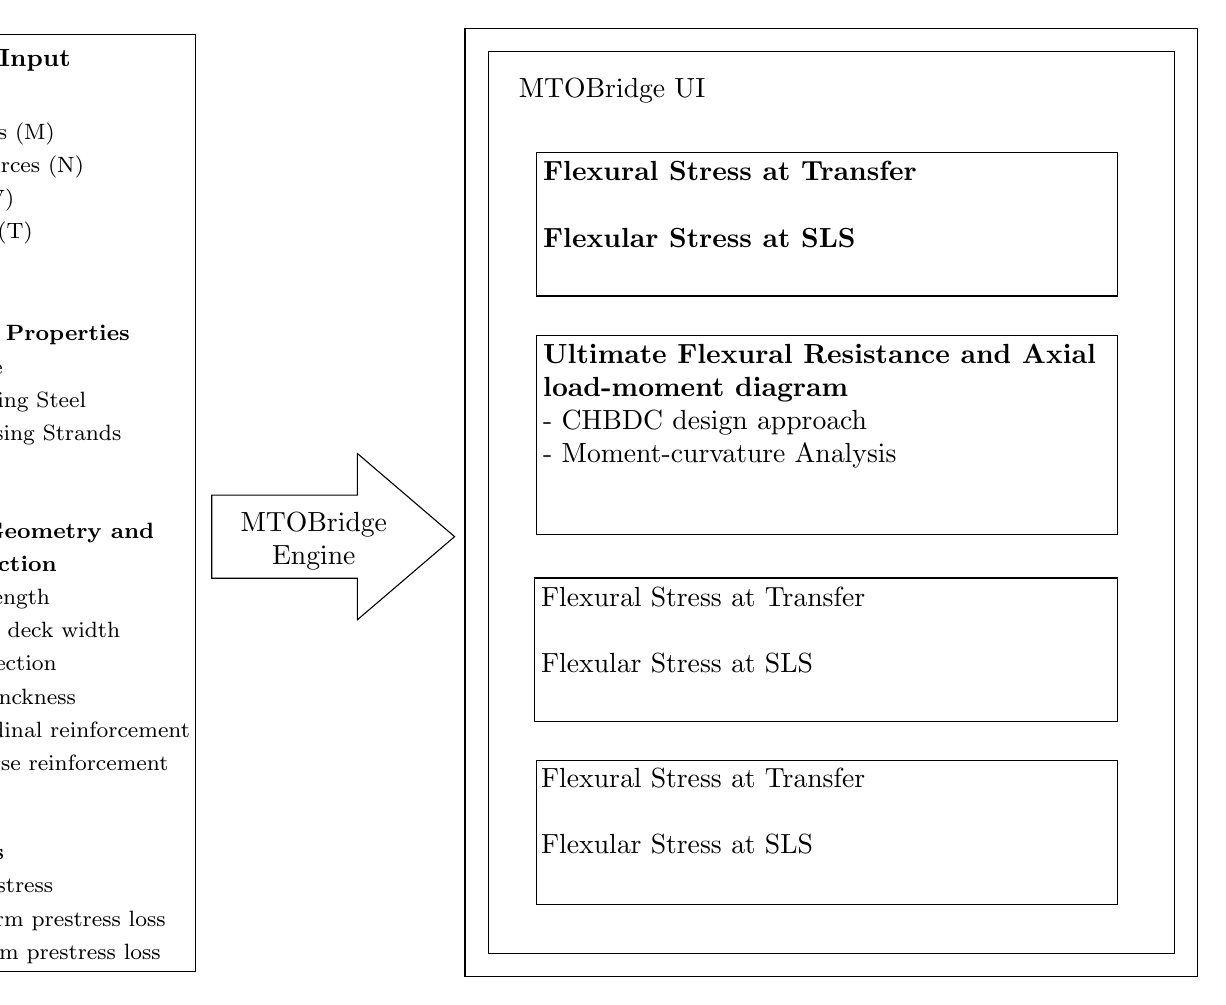
\begin{tikzpicture}[x=0.75pt,y=0.75pt,yscale=-1,xscale=1,trim left=2cm]
%\path (200,200); %set diagram left start at 0, and has height of 554

%Shape: Rectangle [id:dp40713623006932687] 
\draw   (9.8,30.81) -- (156.55,30.81) -- (156.55,482.64) -- (9.8,482.64) -- cycle ;
%Right Arrow [id:dp022223857966380267] 
\draw   (164.55,252.93) -- (234.75,252.93) -- (234.75,232.91) -- (281.55,272.95) -- (234.75,313) -- (234.75,292.98) -- (164.55,292.98) -- cycle ;
%Shape: Rectangle [id:dp6440046928241534] 
\draw   (321,87.9) -- (601,87.9) -- (601,157) -- (321,157) -- cycle ;
%Shape: Rectangle [id:dp15284232981487356] 
\draw   (321,175.9) -- (601,175.9) -- (601,272) -- (321,272) -- cycle ;
%Shape: Rectangle [id:dp9132870930202315] 
\draw   (320,292.9) -- (601,292.9) -- (601,362) -- (320,362) -- cycle ;
%Shape: Rectangle [id:dp5415191968439061] 
\draw   (321,380.9) -- (601,380.9) -- (601,450) -- (321,450) -- cycle ;

%Shape: Frame [id:dp281589755928753] 
\draw   (286.55,28) -- (639.55,28) -- (639.55,485) -- (286.55,485) -- cycle(628.23,39.32) -- (297.86,39.32) -- (297.86,473.68) -- (628.23,473.68) -- cycle ;

\draw (60.8,36.81) node [anchor=north west][inner sep=0.75pt]   [align=left] {\textbf{{\small Input}}};
% Text Node
\draw (11.8,56.81) node [anchor=north west][inner sep=0.75pt]   [align=left] {\textbf{{\footnotesize Loads}}\\{\footnotesize - Moments (M) }\\{\footnotesize - Axial Forces (N)}\\{\footnotesize - Shear (V)}\\{\footnotesize - Torsion (T)}};
% Text Node
\draw (11,170) node [anchor=north west][inner sep=0.75pt]   [align=left] {\textbf{{\footnotesize Material Properties}}\\{\footnotesize - Concrete}\\{\footnotesize - Reinforcing Steel}\\{\footnotesize - Prestressing Strands}\\};
% Text Node
\draw (11,265) node [anchor=north west][inner sep=0.75pt]   [align=left] {\textbf{{\footnotesize Girder Geometry and }}\\\textbf{{\footnotesize Cross Section}}\\{\footnotesize - Girder length }\\{\footnotesize - Effective deck width}\\{\footnotesize - Girder section}\\{\footnotesize - Deck thinckness}\\{\footnotesize - Longitudinal reinforcement}\\{\footnotesize - Transverse reinforcement}};
% Text Node
\draw (11,420) node [anchor=north west][inner sep=0.75pt]   [align=left] {\textbf{{\footnotesize Prestress}}\\{\footnotesize - Jacking stress }\\{\footnotesize - Short-term prestress loss}\\{\footnotesize - Long-term prestress loss}};
% Text Node
\draw (176,260) node [anchor=north west][inner sep=0.75pt]   [align=left] {\begin{minipage}[lt]{54.67pt}\setlength\topsep{0pt}
\begin{center}
MTOBridge\\Engine
\end{center}

\end{minipage}};
% Text Node
\draw (311,51) node [anchor=north west][inner sep=0.75pt]   [align=left] {\begin{minipage}[lt]{67.71pt}\setlength\topsep{0pt}
\begin{center}
MTOBridge UI
\end{center}

\end{minipage}};
% Text Node
\draw (323,90.9) node [anchor=north west][inner sep=0.75pt]   [align=left] {\textbf{Flexural Stress at Transfer }\\\\\textbf{Flexular Stress at SLS}};
% Text Node
\draw (323,178.9) node [anchor=north west][inner sep=0.75pt]   [align=left] {\textbf{Ultimate Flexural Resistance and Axial }\\\textbf{load-moment diagram}\\\mbox{-} CHBDC design approach \ \\\mbox{-} Moment-curvature Analysis };
% Text Node
\draw (322,295.9) node [anchor=north west][inner sep=0.75pt]   [align=left] {Flexural Stress at Transfer \\\\Flexular Stress at SLS};
% Text Node
\draw (322,383.09) node [anchor=north west][inner sep=0.75pt]   [align=left] {Flexural Stress at Transfer \\\\Flexular Stress at SLS};


\end{tikzpicture}

\captionof{figure}{\textbf{MTOBridge Data Flow}}

\subsection{Stakeholders}

\begin{itemize}
  \item Ontario Ministry of Transport
  \item Department of Civil Engineering, McMaster
  \item Department of Software Engineering, McMaster 
\end{itemize}
\subsection{Environment}
\begin{itemize}
  \item Compatible with the latest Windows 10 versions (20H1+)
  \item Fully operational offline 
  \item Requires C++ GNU compiler 
\end{itemize}
%\wss{Hardware and software}

\section{Goals}

\section{Stretch Goals}

\end{document}